\documentclass[tikz,border=8pt]{standalone}
% Shared look for every TikZ diagram. Load with \input{../../tools/tikz-style.tex}
\usepackage[sfdefault]{roboto}
\usetikzlibrary{arrows.meta, positioning, shapes.geometric, calc, fit, backgrounds}
\definecolor{cblue}{HTML}{4C78A8}
\definecolor{corange}{HTML}{F58518}
\definecolor{cgreen}{HTML}{54A24B}
\definecolor{cred}{HTML}{E45756}
\definecolor{cpurple}{HTML}{B279A2}
\definecolor{cgrey}{HTML}{6B6B6B}
\tikzset{
  every picture/.style={font=\sffamily, line width=1.2pt},
  box/.style={draw=#1, fill=#1!12, rounded corners=4pt, align=center, inner sep=7pt, minimum height=1.1cm},
  box/.default=cgrey,
  arrow/.style={-{Stealth[length=3mm]}, draw=cgrey, line width=1.4pt},
  title/.style={font=\sffamily\bfseries\Large},
  note/.style={font=\sffamily\small, text=cgrey, align=center},
}
\AtBeginDocument{\hyphenpenalty=10000 \exhyphenpenalty=10000}

% TEB's footprint models (include/teb_local_planner/robot_footprint_model.h, ros2-master; parameter footprint_model.type):
% the distance to an obstacle that the obstacle edges use. point: to the centre; circular: to the centre minus the
% radius; two_circles: the smaller of the two circles' distances; line: to the segment minus a radius; polygon: to the
% outline. The car is RO-055's: 4.0 m x 1.8 m, pose at the middle of the rear axle, 0.75 m from the rear bumper.
\begin{document}
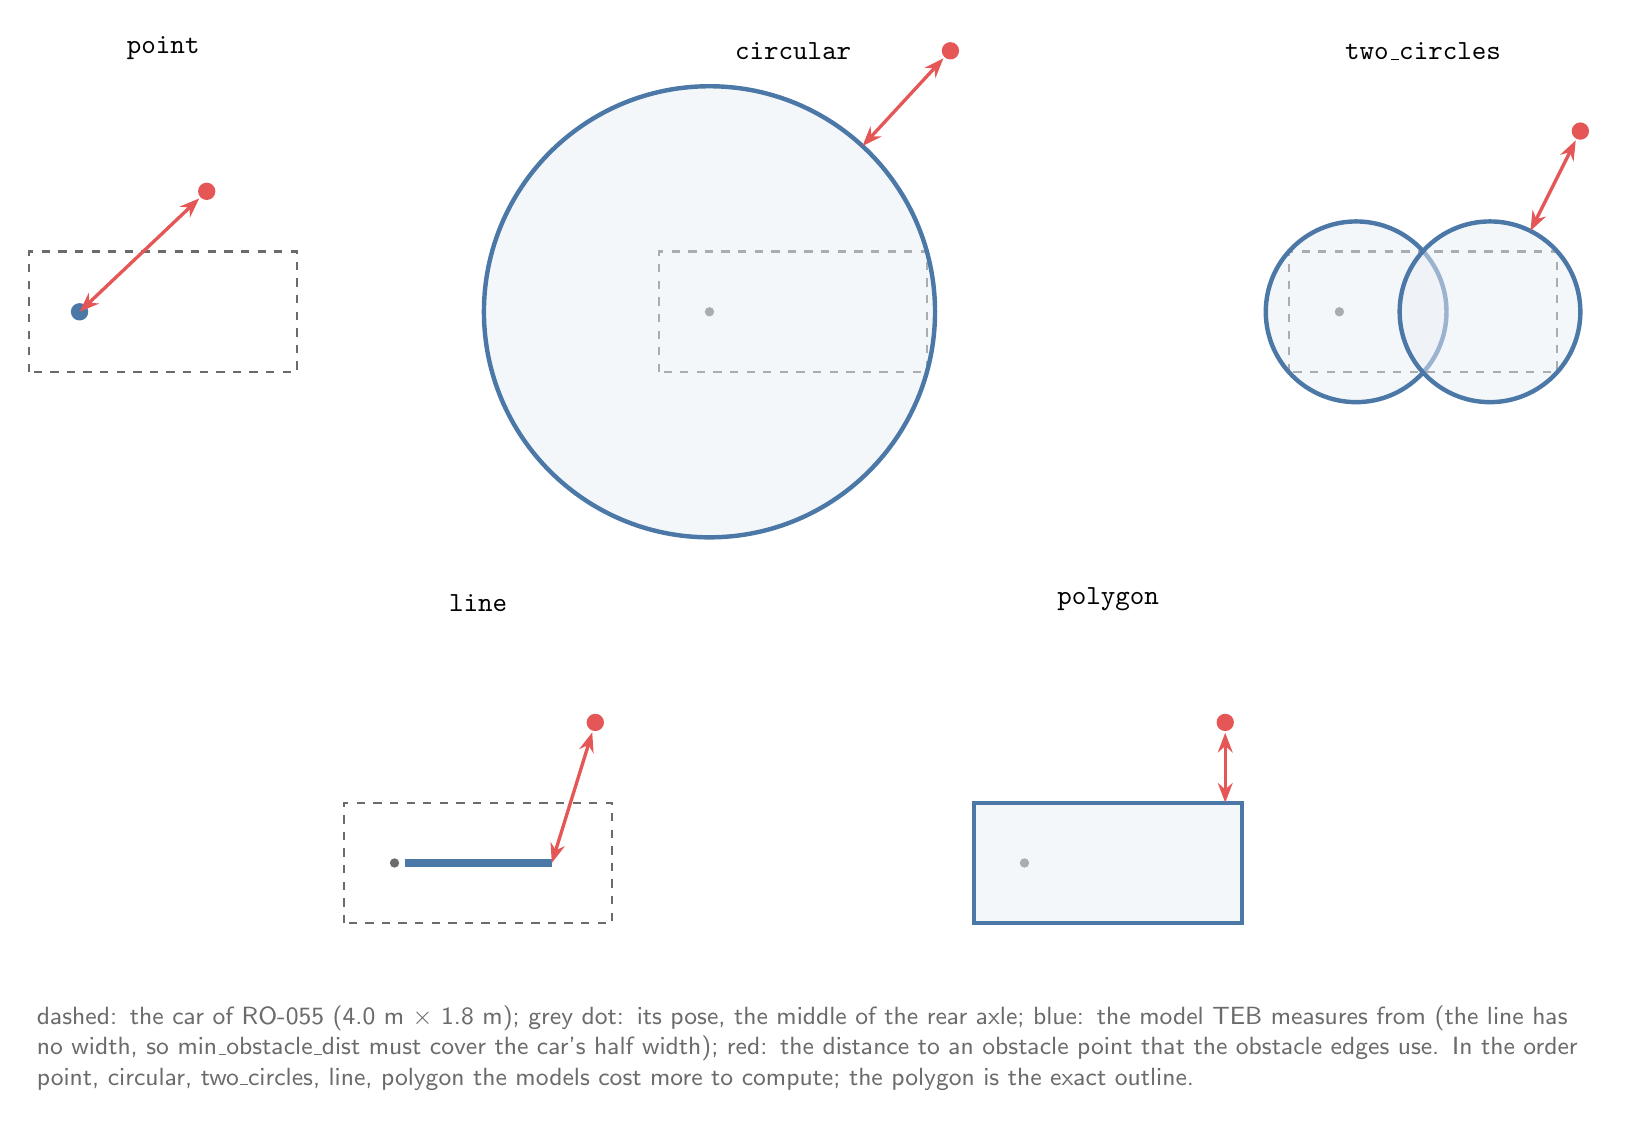
\begin{tikzpicture}[x=0.85cm, y=0.85cm,
  car/.style={draw=cgrey, line width=0.8pt, dashed},
  model/.style={draw=cblue, line width=1.6pt, fill=cblue!12},
  ob/.style={circle, fill=cred, minimum size=0.22cm, inner sep=0pt},
  dist/.style={{Stealth[length=2.5mm]}-{Stealth[length=2.5mm]}, draw=cred, line width=1.2pt},
  ttl/.style={font=\bfseries\normalsize, anchor=south}]
  \foreach \dx/\dy/\name in {0/0/point, 8/0/circular, 16/0/two\_circles, 4/-7/line, 12/-7/polygon} {
    \begin{scope}[xshift=\dx cm, yshift=\dy cm]
      \draw[car] (-0.75,-0.9) rectangle (3.25,0.9);
      \node[ttl] at (1.25,3.6) {\texttt{\name}};
      \fill[cgrey] (0,0) circle (0.07);
    \end{scope}
  }
  % point
  \begin{scope}[xshift=0cm]
    \fill[cblue] (0,0) circle (0.13);
    \node[ob] (o) at (1.9,1.8) {};
    \draw[dist] (0,0) -- (o);
  \end{scope}
  % circular: centred on the pose (the rear axle); 3.37 m reaches the front corners
  \begin{scope}[xshift=8.0cm]
    \draw[model, fill opacity=0.5] (0,0) circle (3.37);
    \node[ob] (o) at (3.6,3.9) {};
    \draw[dist] ($(0,0)!2.8645cm!(o)$) -- (o);
  \end{scope}
  % two circles
  \begin{scope}[xshift=16.0cm]
    \draw[model, fill opacity=0.5] (0.25,0) circle (1.35);
    \draw[model, fill opacity=0.5] (2.25,0) circle (1.35);
    \node[ob] (o) at (3.6,2.7) {};
    \draw[dist] ($(2.25,0)!1.1475cm!(o)$) -- (o);
  \end{scope}
  % line: zero width; min_obstacle_dist must cover the half width
  \begin{scope}[xshift=4cm, yshift=-7cm]
    \draw[cblue, line width=2.6pt] (0.15,0) -- (2.35,0);
    \node[ob] (o) at (3.0,2.1) {};
    \draw[dist] (2.35,0) -- (o);
  \end{scope}
  % polygon
  \begin{scope}[xshift=12cm, yshift=-7cm]
    \draw[model, fill opacity=0.5] (-0.75,-0.9) rectangle (3.25,0.9);
    \node[ob] (o) at (3.0,2.1) {};
    \draw[dist] (3.0,0.9) -- (o);
  \end{scope}
  \node[note, anchor=west, text width=20cm, align=left] at (-0.8,-11.0) {dashed: the car of RO-055 (4.0 m $\times$ 1.8 m); grey dot: its pose, the middle of the rear axle; blue: the model TEB measures from (the line has no width, so min\_obstacle\_dist must cover the car's half width); red: the distance to an obstacle point that the obstacle edges use. In the order point, circular, two\_circles, line, polygon the models cost more to compute; the polygon is the exact outline.};
\end{tikzpicture}
\end{document}
